\documentclass{article}
\usepackage{amsmath,amsthm,amssymb}
\usepackage{mathtext}
\usepackage[T2A]{fontenc}
\usepackage[utf8]{inputenc}
\usepackage[english]{babel}
\usepackage{graphicx}
\usepackage{hyperref}


\title{Stock Market Prediction Using News Articles}
\author{Ruslan Sirazhetdinov} 

\date{May 2023}



\begin{document}
\maketitle
\begin{abstract}
    
    
    This document will provide you with guidelines for your project final report. You will learn how to structure the report and present your results. Use this field for the short description of your work. Please provide a link to your project code right here: \url{https://github.com/irusland/nlpystocks}.
\end{abstract}



\section{Introduction}
The topic of predicting stock market using NLP techniques 


First of all, you will need to write the whole report in English, with a few exceptions mentioned below.
This section is devoted to a problem motivation. You should answer the question of why the problem you were working on is important. Also, you should describe what is unique in your approach to this problem, what are the differences to other approaches.
\subsection{Team}
\textbf{Sirazhetdinov Ruslan} \href{mailto:sirazhetdinov.rr@phystech.edu}{sirazhetdinov.rr@phystech.edu}

I was the only one participant in the team and responsible for several goals:

\begin{enumerate}
  \item  determination of current state of the art solutions and related works.
  \item  researching the topic of existing datasets that will suit the need of this work.
  \item  preparation of news and stocks dataset, with custom human-like crawler.
  \item  making a simple baseline solution.
  \item  adapting existing models from related works for dataset.
  \item  implementation of proposed solution.
  
\end{enumerate}


\section{Related Work}
\label{sec:related}
I was not able to find a suitable source code for related work solutions, some haven't provided a source code links, and others have been implemented in different programming languages like java, 
Since i am using python as a tool in this research, i have tried to implement my own representation according to experiment notes in papers.

In this section, you will describe in details the existing approaches to the problem you work on. For each approach, you need to provide a reference. 

\cite{levenshtein1966binary} is a sample reference to the previous art. \cite{levenshtein1966dvoichnie} is a sample reference in Russian.

\section{Model Description}
Here you need to write a detailed description of your approach. It is important to mention that this description should give more details than the descriptions from section \ref{sec:related}\footnote{This is an example of internal references and footnotes at the same time.}. 

You will likely be providing a figure to better present your approach. A sample circle is presented on Fig.~\ref{fig:circle}.

The other possible contents of this section are formulae. They could be on a new line:
$$S=\pi r^2,$$
or they could be inline, e.g. if you want to describe the used variables, like $S$ is an area of a circle, while $r$ is its radius. 

\begin{figure}[!tbh]
    \centering
    
\includegraphics[width=0.3\linewidth]{circle.png}
    \caption{A sample circle.}
    \label{fig:circle}
\end{figure}

\section{Dataset}

For the task of predicting stock market i needed a dataset with news articles and current market state.
I have researched for avalable datasets, and there where plenty of twitter's related ones.
I wanted to experiment on Russian stock market via using Russian news. 
And specifically, i did not chose the existing news datasets because they were too broad on topics. My goal was to process only financial related articles.
So my choice was the Finam's newsline\footnote{Raw content from Finam's newline could be found ~\href{https://www.finam.ru/publications/selection/united/}{here}.} also i was their client.

I should mention that, it was not easy to get it downloaded. 
My first naive approach was to just load it using \href{https://pypi.org/project/requests/}{python requests}. But it turned out that they had an interface, where you need to click on the button in order to load another portion of news. So i discovered \href{https://pypi.org/project/selenium/}{python selenium}, a new approach to emulate human-like gestures and button clicks on the web page.

The notebook \texttt{/notebooks/news-scraping.ipynb} consist of scraping a web page with news.

It is important to mention that the dataset is available for the research purposes. 
Finam does allow to use the information with giving a link to in according to \href{https://www.finam.ru/about/copyright/}{copyright policy}

The second stage in the notebook \texttt{/notebooks/stocks-dataset.ipynb} was to load a stock market values from stock exchange. 
As an employee of Tinkoff bank and an active contributor of \href{https://github.com/Tinkoff/invest-python}{invest-python library} i used the Tinkoff Investments OpenAPI \footnote{Tinkoff Invest OpenAPI could be found ~\href{https://www.tinkoff.ru/invest/open-api/}{here}.} to load the Sberbank privileged shares with FIGI number \texttt{BBG0047315Y7} for the period of previous year. I chose the Sberbank shares instrument because it has high liquidity and high volatility. I believe that such instrument is quite popular among investors.

Having to separate datasets I have joined them together by matching a \texttt{date} column that contained current date. 
See the details in \texttt{notebooks/dataset.ipynb}.

I represent some statistics of resulting StocksNews dataset on Tab.~\ref{tab:statistics} The dataset was split into two parts: train and test with proportion of 88/22 percent accordingy. It's important to mention that this is a time series dataset so I did not use any king of shuffling. 

\begin{table}[tbh!]
\begin{center}
\begin{tabular}[t]{|l|cc|}
\hline
%\cline{2-4}
 & Train & Test \\
\hline
Proportion & 0.88 & 0.22  \\
Size & 23879 & 6735 \\
Vocabulary size & \multicolumn{2}{c|}{16507} \\
Date range & 2022.05.08 - 2023.02.10 & 2023.02.10 - 2023.05.06 \\

\hline
\end{tabular}
\caption{Statistics of the StocksNews dataset. The out of vocabulary (OoV) rate notes what percentage of tokens have been replaced by an $\langle unk \rangle$ token. The token count includes newlines which add to the structure of the dataset.}
\label{tab:statistics}
\end{center}
\end{table}

\begin{figure}[!tbh]
    \centering
    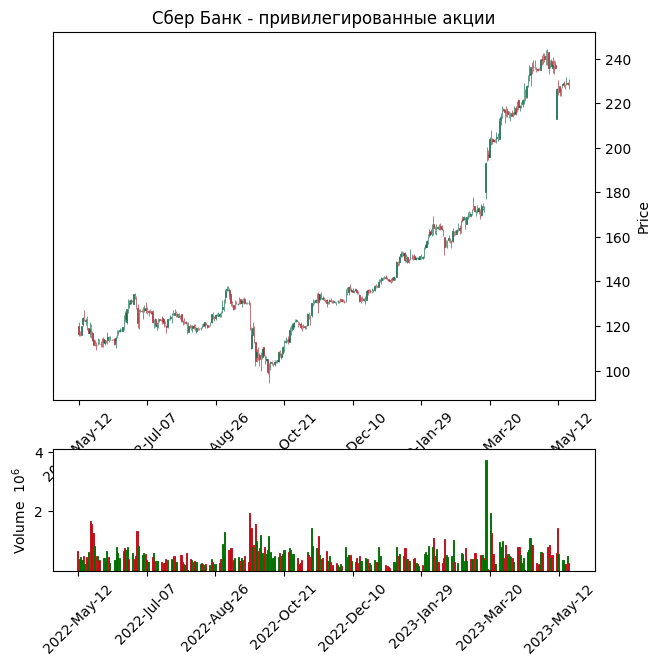
\includegraphics[width=0.3\linewidth]{sber.png}
    \caption{Sberbank shares cost values in dataset.}
    \label{fig:sber}
\end{figure}

When constructing a baseline with TF-IDF\footnote{TF-IDF model to get the sentence embeddings. Details at ~\href{https://ru.wikipedia.org/wiki/TF-IDF}{Wikipedia}.} embeddings, I have used. -------- написать про яндекс лемма

It's worth mentioning that the using the other dataset preprocessing techniques have not been done and could be other possible research topics which is out of scope of current.

If you were collecting the dataset on your own please describe the collection procedure, like criteria were used to filter the documents, the pre-processing steps, etc. It is preferable that you release your dataset for the public, but you are not obliged to do this. Please make sure that you have legal rights to collect and distribute the data you were working with. We recommend you to look at C4Corpus and how it is licensed to make your corpora. C4Corpus is described in~\cite{habernal2016c4corpus}.

\section{Experiments}
This section should include several subsections.
\subsection{Metrics}
First of all, you should describe the metric(s) you were using to evaluate your approach. Most likely a metric description will include a formula.

\subsection{Experiment Setup}
Secondly, you need to describe the design of your experiment, e.g. how many runs there were, how the data split was done. The important details of your model, like hyper-parameters used in the experiments, and so on.

\subsection{Baselines}
Another important feature is that you could provide here the description of some simple approaches for your problem, like logistic regression over TF-IDF embedding for text classification. The baselines are needed is there is no previous art on the problem you are presenting.

\section{Results}
In this section, you need to list and describe the achieved results. It is crucial to have the results of the experiments for the other approaches. This is needed to be able to compare your results with some competitors. Most preferably, you should provide some references with results on the same problem.

Almost inevitably the results are presented as a table, but it is also possible to have a graph, i.e. a figure.

You need also to provide an interpretation of the presented results, to describe some features. E.g. your approach shows higher results on the short texts or by one metric instead of another.

Also in this section, you could provide some results for your model inference. The samples could be found in Tab.~\ref{tab:output}.

\begin{table}[!tbh]
    \centering
    \begin{tabular}{|c|}
\hline
Это пример вывода вашей модели на русском.\\
This is a sample output of your model in English.
\\
\hline
    \end{tabular}
    \caption{Output samples.}
    \label{tab:output}
\end{table}

\section{Conclusion}
In this section, you need to describe all the work in short: what you have done and what has been achieved. E.g. you have collected a dataset, made a markup for it and developed a model showing the best results compared to other models. 

\bibliographystyle{apalike}
\bibliography{lit}
\end{document}
